\documentclass[a4paper]{article}
\usepackage{amsmath}
\usepackage{graphicx}
\begin{titlepage}
  \title{Report project 2 IT3708}
  \author{Lars Andersen \\
    Tormund S. Haus}
  \date{\today}
\end{titlepage}

\begin{document}
\maketitle

\section{Introduction}
\label{sec:introduction}

In this report we will detail the changes we made to our evolutionary algorithm system, EASY, to solve the second assignment.

We will then show how we used EASY to solve the second assignment. Specifically, we will take a close look at the genotype selection and the fitness functions.

12 test cases were provided with assignment two and we'll see how close EASY is able to get to the target spike trains. This will include some gritty details about the evolutionary algorithm, EA, parameters used.

Finally, there will a discussion about the genotype to phenotype mapping, the practical implications of this tool and of other domains where a more general version of this tool might be put to use.

\section{System overview}
\label{sec:system_overview}

We went to great lengths--nearly choking on generics--in order to make EASY as general as humanly possible. Because of our previous efforts it was very straight forward to use the system in order to solve a new problem. All we had to do was:

\begin{itemize}
\item Add a new neuron individual.
\item Add classes for the different fitness metrics.
\item Create a new Report class.
\item Make new Replicator and Incubator class.
\end{itemize}

This might sound like a lot of code, but it really isn't. The individual class was able to inherit almost all of its functionality from AbstractIndividual. We also pushed quite a bit of code up to a newly created AbstractIncubator class. The effect was that the new NeuronIncubator class, the class responsible for making new Individuals, was only some ten lines of code long!

GNUPlot is pretty great, but it can be a bit of a pain to call it from a Java program. To make this easier someone has written an interface to GNUPlot called JavaPlot. We're going to make use of this library for this assignment in order to make it easier for ourselves to create plots.

Otherwise, we've made quite a few bugfixes as well. These bugs weren't apparent with the previous input data, but caused the system to halt when we first attempted to use it on the new data. The system should be a bit more robust now, and our defensive programming skills improved.

\subsection{Genotype}
\label{sec:genotype}

We're using the same type of genotype as we used to solve the Blotto problem: a vector of doubles. In this case the vector has a length of 5 and contains all the parameters for the Itzhikevich neuron model.

We're using a random sample from a gaussian of mean 0 in order to mutate the values. Because the parameters for the neuron model have different ranges we're scaling the amplitude of the Gaussian distribution to match this.

We're using Random.nextGaussian(), from the Java standard library to do this. This function doesn't allow you to set the variance. Being unable to set the variance caused us some problems because values above $\pm$1 are too likely to occur. Our solution to limit the amplitude of the Gaussian is satisfactory, but it would've been prettier if we implemented our own Gaussian and set the variance ourselves. At first values outside the range (when the scaled Gaussian returned values above $\pm$1) were mapped to $MAX$ and $MIN$, but we later changed this to simply generate another number. The latter approach is definitely better, and it doesn't happen often enough to limit performance.

\subsection{Fitness functions}
\label{sec:fitfuncs}

The different fitness functions are:

\begin{equation}
  \label{eq:1}
  F_m = \frac{1}{1+d_m}
\end{equation}

\noindent where $F_m$ is the fitness value using distance measure $m$ to produce distance $d_m$. Using \eqref{eq:1} is a natural way to map a distance measure to a fitness value in the interval $[0,1]$. When we're using the spike interval distance measure and spike time distance measure, to calculate distance, we're also applying the recommended penalty, comparing the number of spikes in the two spike trains. This penalty is added to the distance, prior to normalization.

\newpage
\section{Results}

The specific parameters for each run can be found in the zip file, in the log. We apologize that we're running out of time and that the comments in this section will be rather brief.
\label{sec:results}

\begin{figure}[htb!]
  \centering
  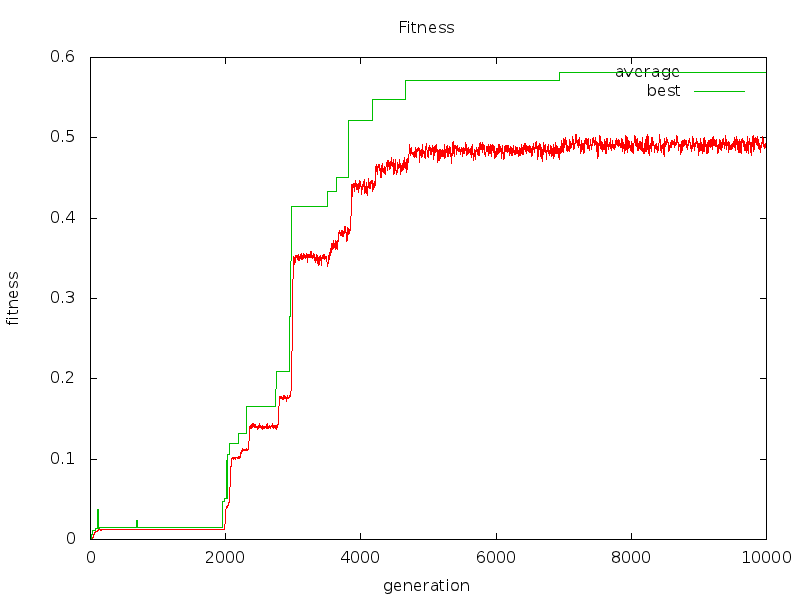
\includegraphics[width=\textwidth]{SpikeTime-izzy1-fitness-plot.png}
  \caption{Fitness Izzy-train1 using Spike time distance measure.}
\end{figure}

Gradual improvement here in figure1, but unable to find the optimal solution.

\begin{figure}[htb!]
  \centering
  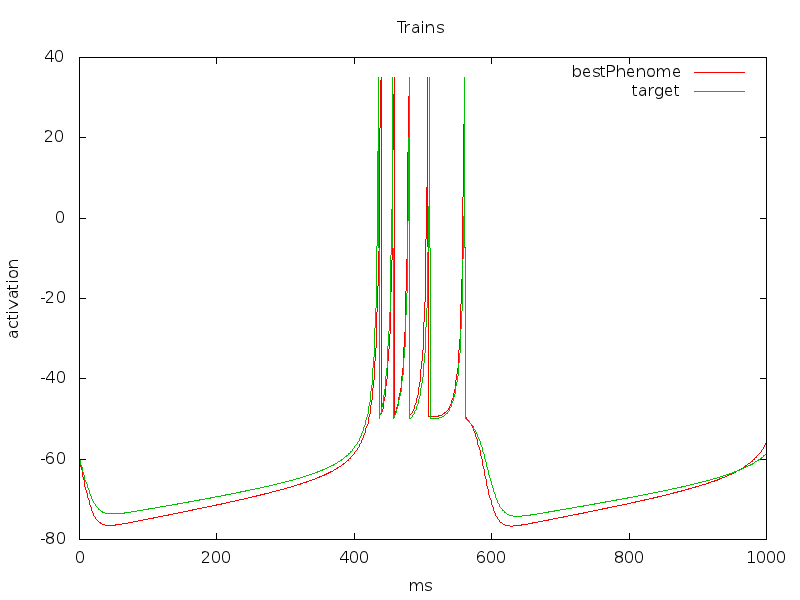
\includegraphics[width=\textwidth]{SpikeTime-izzy1-trains-plot.png}
  \caption{Spike trains for izzy-train1 using spike time distance measure.}
\end{figure}

The spike trains are incredibly similar, just a little bit is missing for a perfect match!

\newpage

\begin{figure}[htb!]
  \centering
  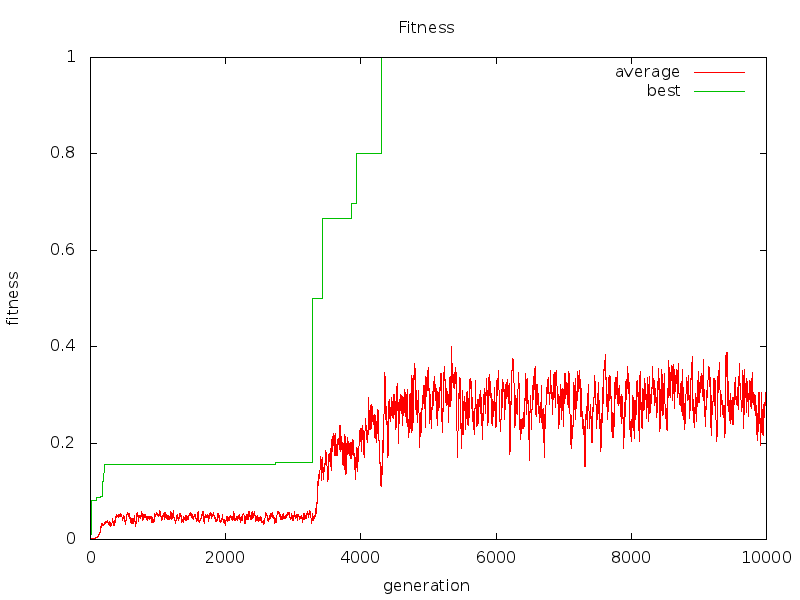
\includegraphics[width=\textwidth]{SpikeInterval-izzy1-fitness-plot.png}
  \caption{Fitness Izzy-train1 using spike time interval distance measure.}
\end{figure}

Here, in figure2, we can see typical behaviour of the system, it's stuck with the same solution for a very long
time until manages to find a new local maximum and then finally the global maximum.

\begin{figure}[htb!]
  \centering
  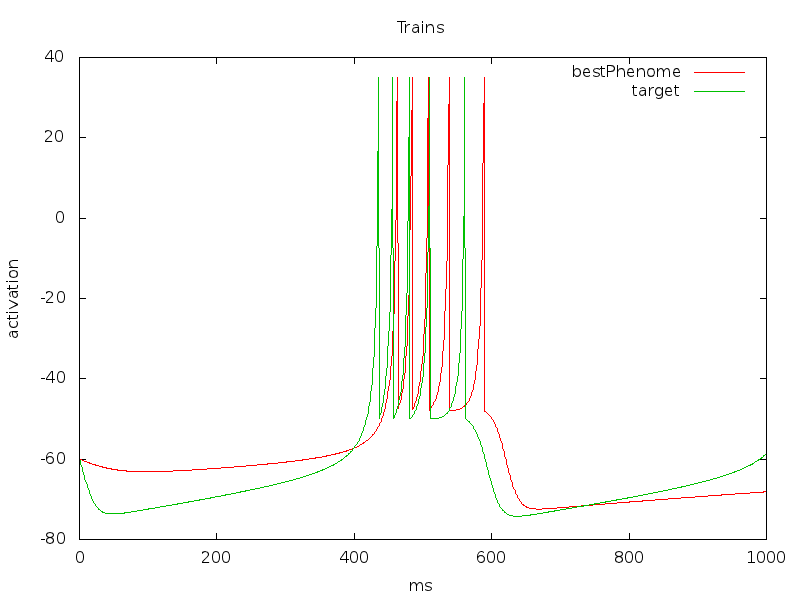
\includegraphics[width=\textwidth]{SpikeInterval-izzy1-trains-plot.png}
  \caption{Spike trains for izzy-train1 using spike interval distance measure.}
\end{figure}

Again the spike trains, as seen in figure4, are very similar, but a little bit is missing. This little bit probably amounts to a huge movement in genotype space, and the system is unable to get there without the individuals dying on the way.

\newpage

\begin{figure}[htb!]
  \centering
  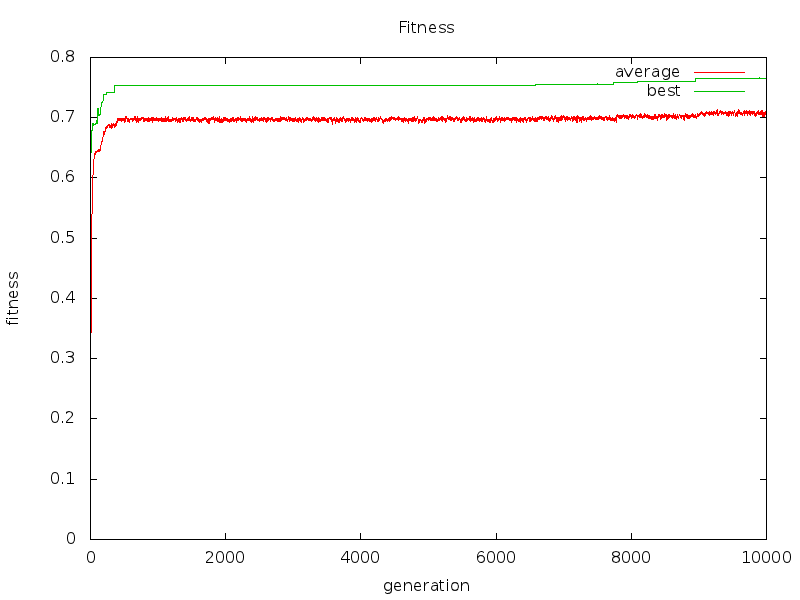
\includegraphics[width=\textwidth]{Waveform-izzy1-fitness-plot.png}
  \caption{Fitness Izzy-train1 using spike time interval distance measure.}
\end{figure}

Local maximum is quickly found in figure5, only small improvements made from there.

\begin{figure}[htb!]
  \centering
  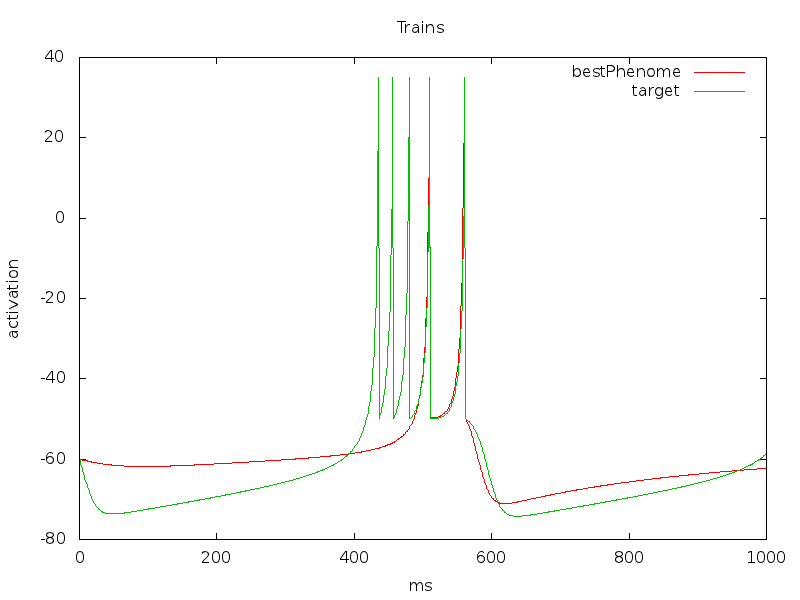
\includegraphics[width=\textwidth]{Waveform-izzy1-trains-plot.png}
  \caption{Spike trains for izzy-train1 using spike interval distance measure.}
\end{figure}

The waveforms in figure6 really aren't as similar as the other ones. But it's pretty clear that a sub-solution has been found.

\newpage

\begin{figure}[htb!]
  \centering
  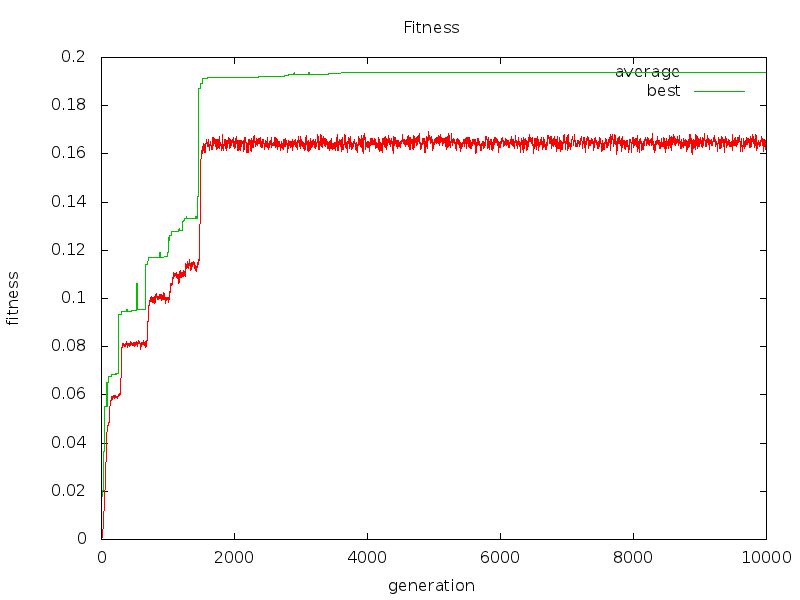
\includegraphics[width=\textwidth]{SpikeTime-izzy2-fitness-plot.png}
  \caption{Fitness Izzy-train2 using Spike time distance measure.}
\end{figure}

\begin{figure}[htb!]
  \centering
  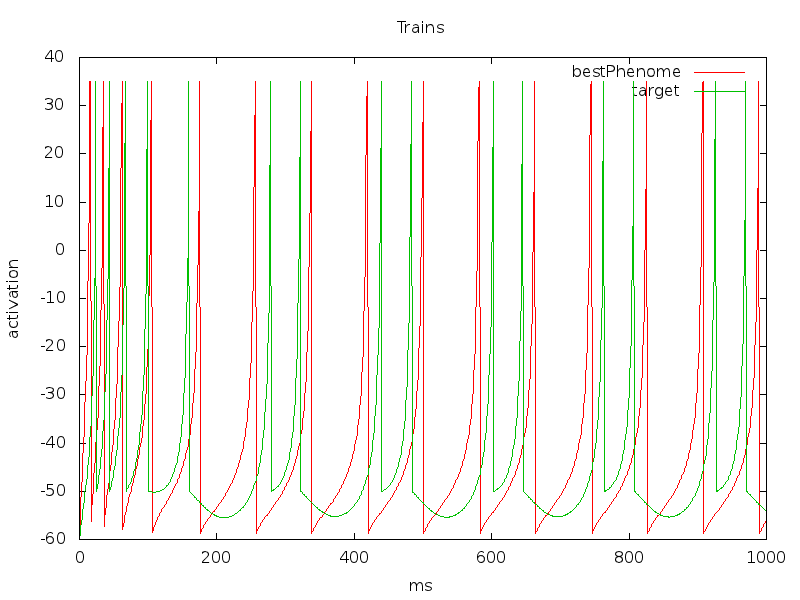
\includegraphics[width=\textwidth]{SpikeTime-izzy2-trains-plot.png}
  \caption{Spike trains for izzy-train2 using spike time distance measure.}
\end{figure}

The spike train here isn't entirely bad, the solution is pretty close!

\newpage

\begin{figure}[htb!]
  \centering
  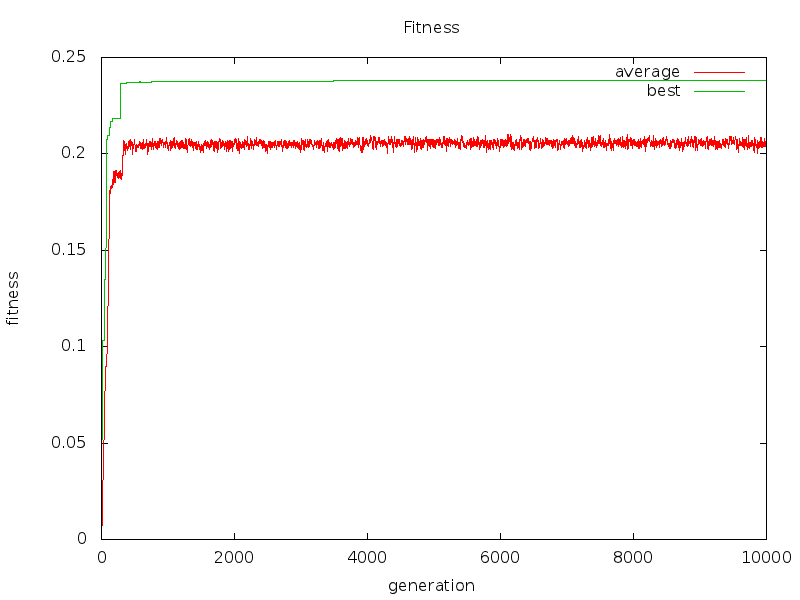
\includegraphics[width=\textwidth]{SpikeInterval-izzy2-fitness-plot.png}
  \caption{Fitness Izzy-train2 using spike time interval distance measure.}
\end{figure}

\begin{figure}[htb!]
  \centering
  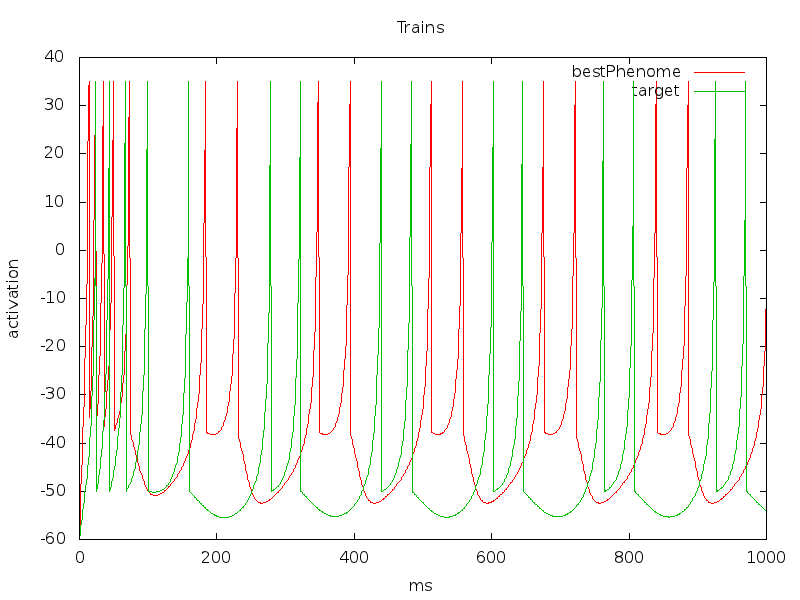
\includegraphics[width=\textwidth]{SpikeInterval-izzy2-trains-plot.png}
  \caption{Spike trains for izzy-train2 using spike interval distance measure.}
\end{figure}

\newpage

\begin{figure}[htb!]
  \centering
  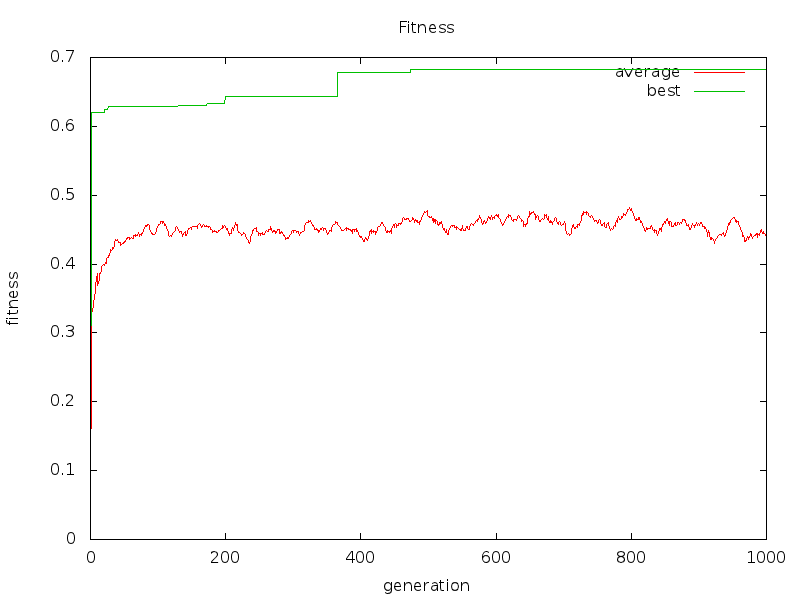
\includegraphics[width=\textwidth]{Waveform-izzy2-fitness-plot.png}
  \caption{Fitness Izzy-train2 using spike time interval distance measure.}
\end{figure}

\begin{figure}[htb!]
  \centering
  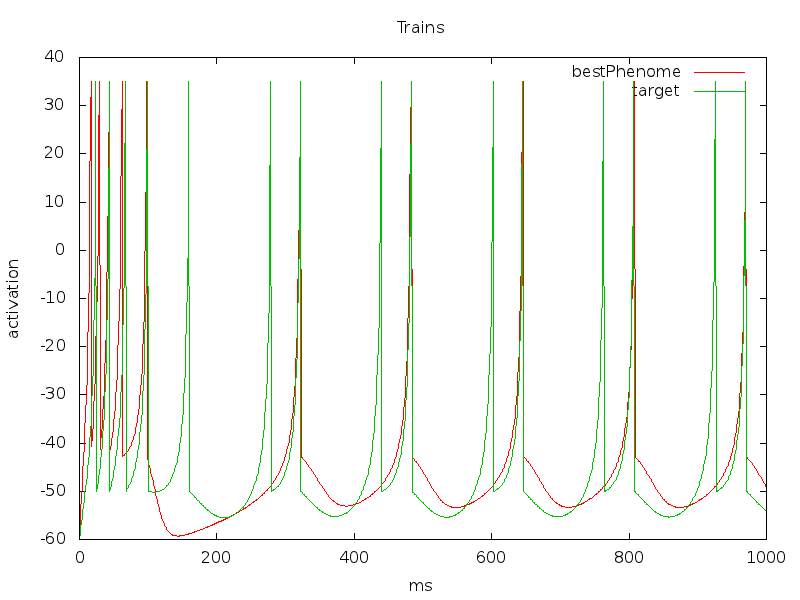
\includegraphics[width=\textwidth]{Waveform-izzy2-trains-plot.png}
  \caption{Spike trains for izzy-train2 using spike interval distance measure.}
\end{figure}

\newpage

\begin{figure}[htb!]
  \centering
  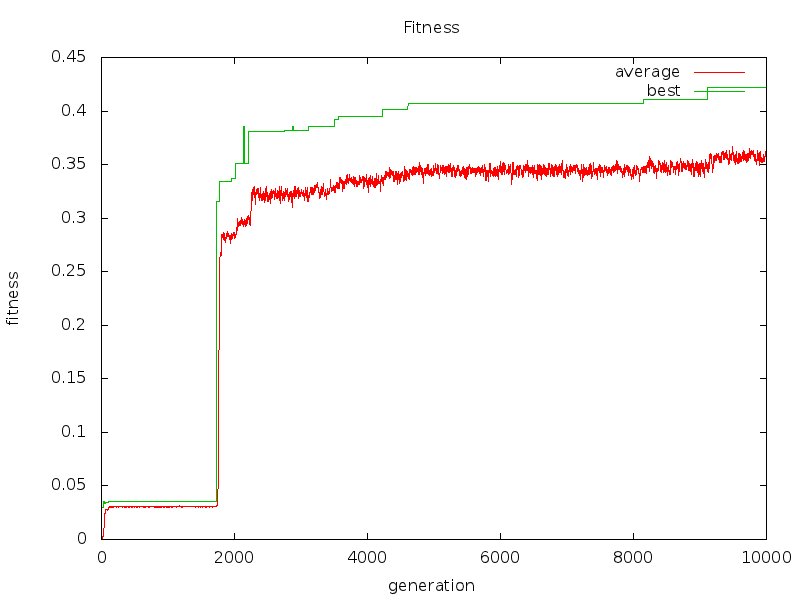
\includegraphics[width=\textwidth]{SpikeTime-izzy3-fitness-plot.png}
  \caption{Fitness Izzy-train3 using Spike time distance measure.}
\end{figure}

\begin{figure}[htb!]
  \centering
  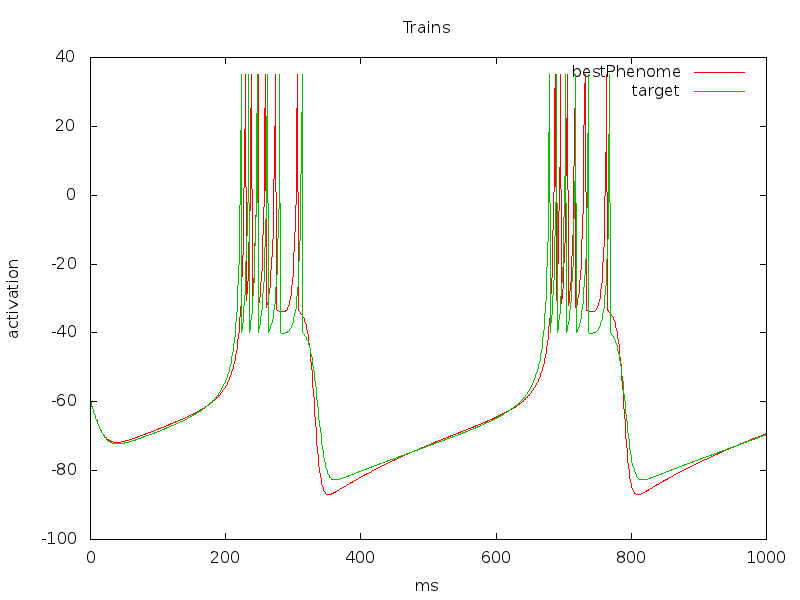
\includegraphics[width=\textwidth]{SpikeTime-izzy3-trains-plot.png}
  \caption{Spike trains for izzy-train3 using spike time distance measure.}
\end{figure}

\newpage

\begin{figure}[htb!]
  \centering
  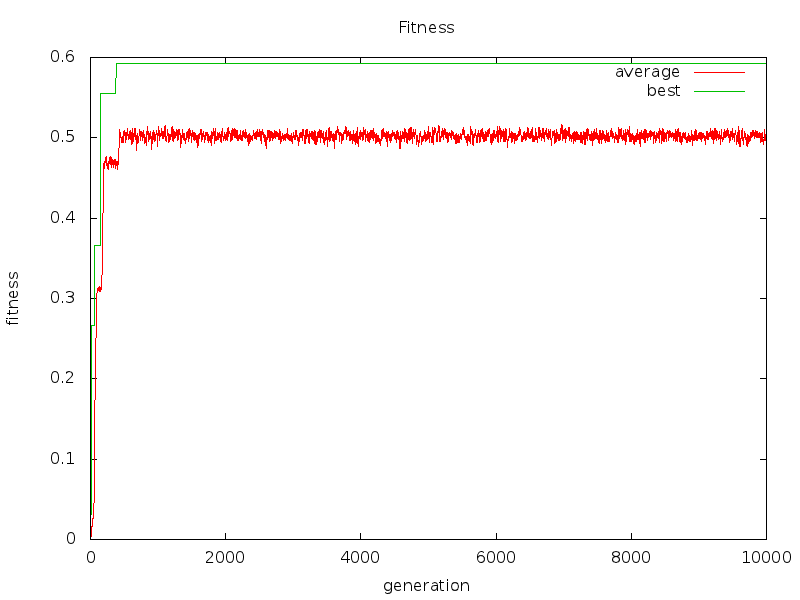
\includegraphics[width=\textwidth]{SpikeInterval-izzy3-fitness-plot.png}
  \caption{Fitness Izzy-train3 using spike time interval distance measure.}
\end{figure}

\begin{figure}[htb!]
  \centering
  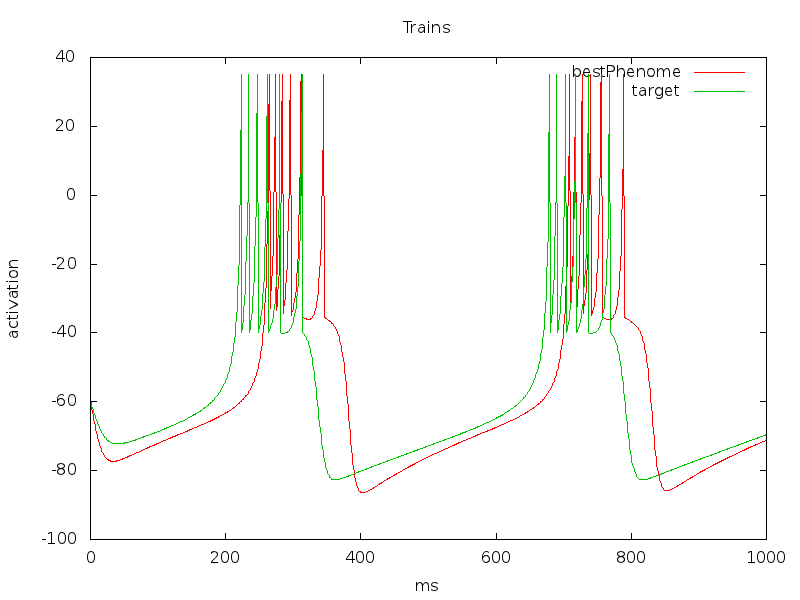
\includegraphics[width=\textwidth]{SpikeInterval-izzy3-trains-plot.png}
  \caption{Spike trains for izzy-train3 using spike interval distance measure.}
\end{figure}

\newpage

\begin{figure}[htb!]
  \centering
  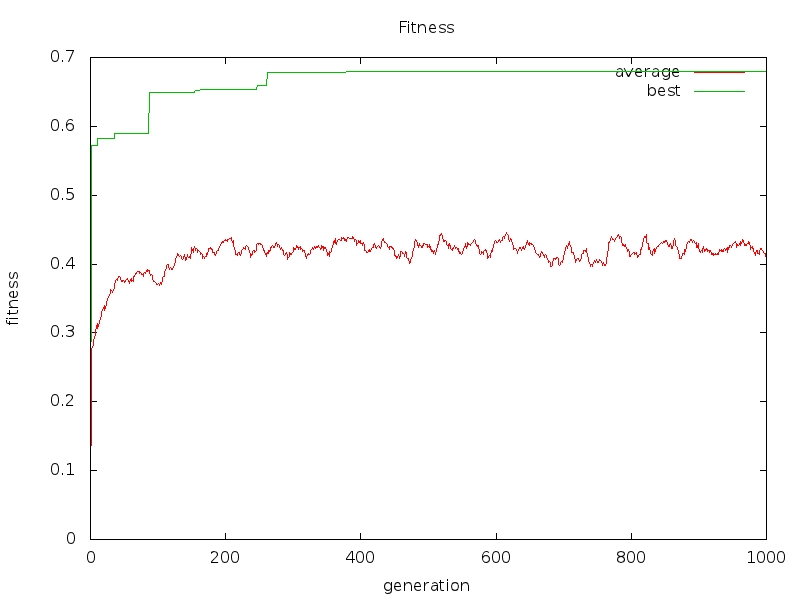
\includegraphics[width=\textwidth]{Waveform-izzy3-fitness-plot.png}
  \caption{Fitness Izzy-train3 using spike time interval distance measure.}
\end{figure}

\begin{figure}[htb!]
  \centering
  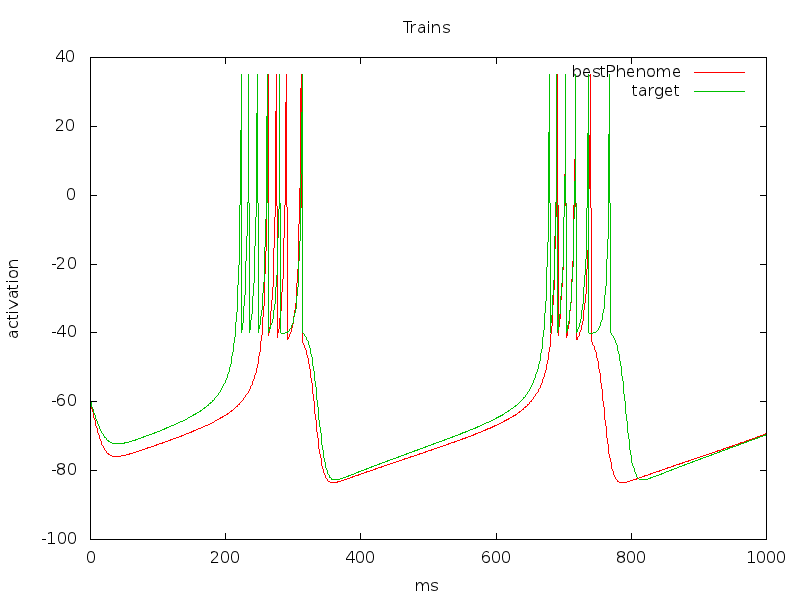
\includegraphics[width=\textwidth]{Waveform-izzy3-trains-plot.png}
  \caption{Spike trains for izzy-train3 using spike interval distance measure.}
\end{figure}

\newpage

\begin{figure}[htb!]
  \centering
  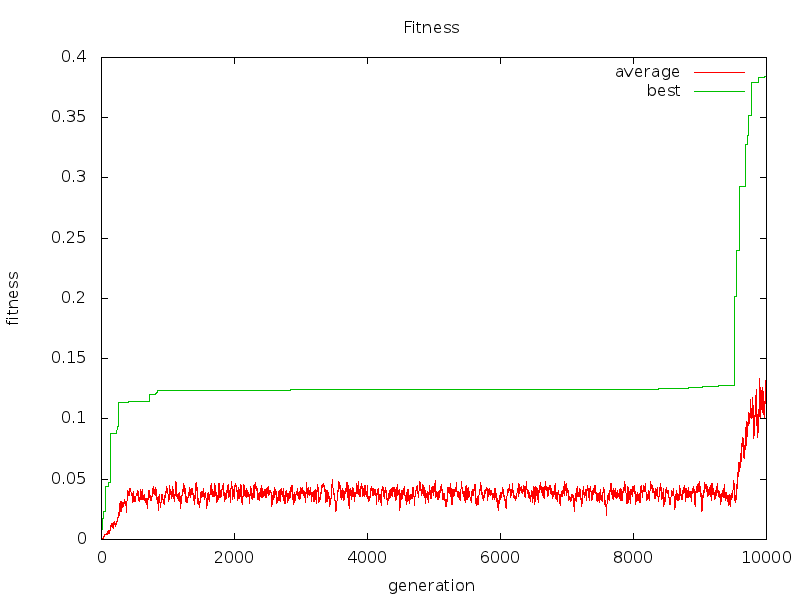
\includegraphics[width=\textwidth]{SpikeTime-izzy4-fitness-plot.png}
  \caption{Fitness Izzy-train4 using Spike time distance measure.}
\end{figure}

\begin{figure}[htb!]
  \centering
  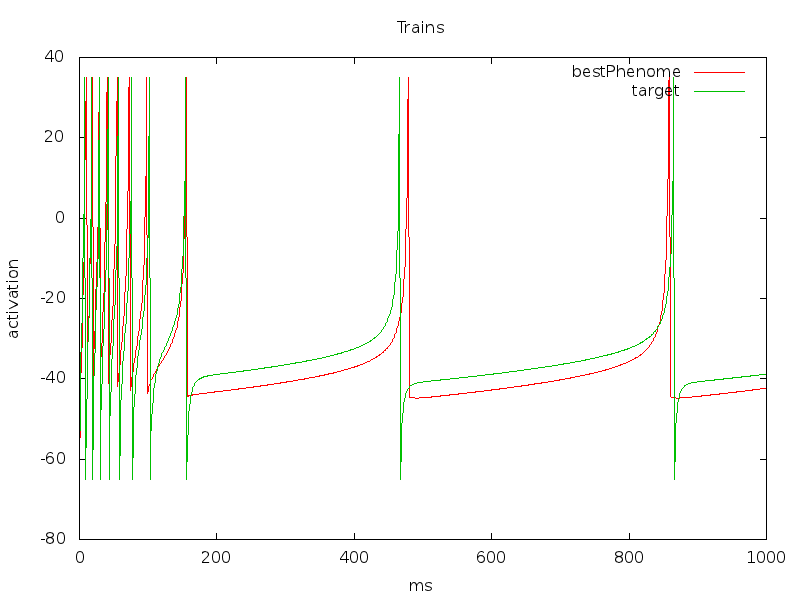
\includegraphics[width=\textwidth]{SpikeTime-izzy4-trains-plot.png}
  \caption{Spike trains for izzy-train4 using spike time distance measure.}
\end{figure}

\newpage

\begin{figure}[htb!]
  \centering
  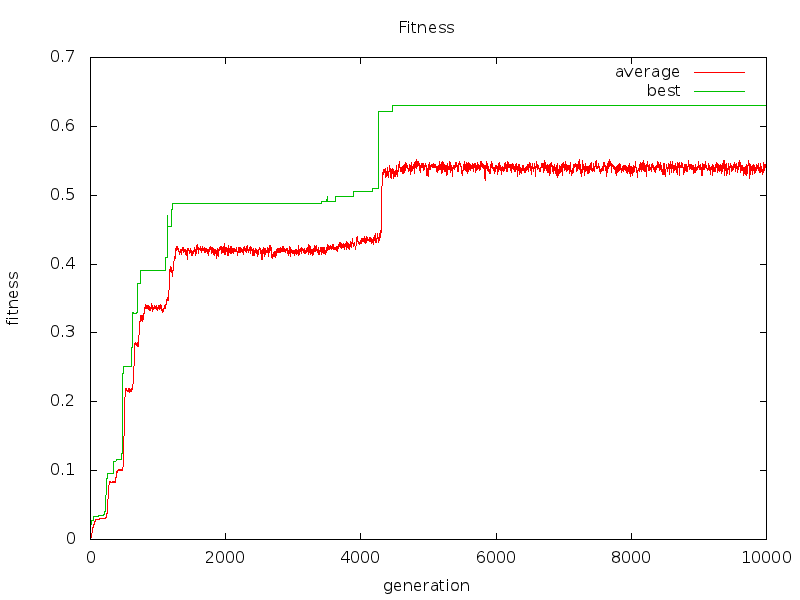
\includegraphics[width=\textwidth]{SpikeInterval-izzy4-fitness-plot.png}
  \caption{Fitness Izzy-train4 using spike time interval distance measure.}
\end{figure}

\begin{figure}[htb!]
  \centering
  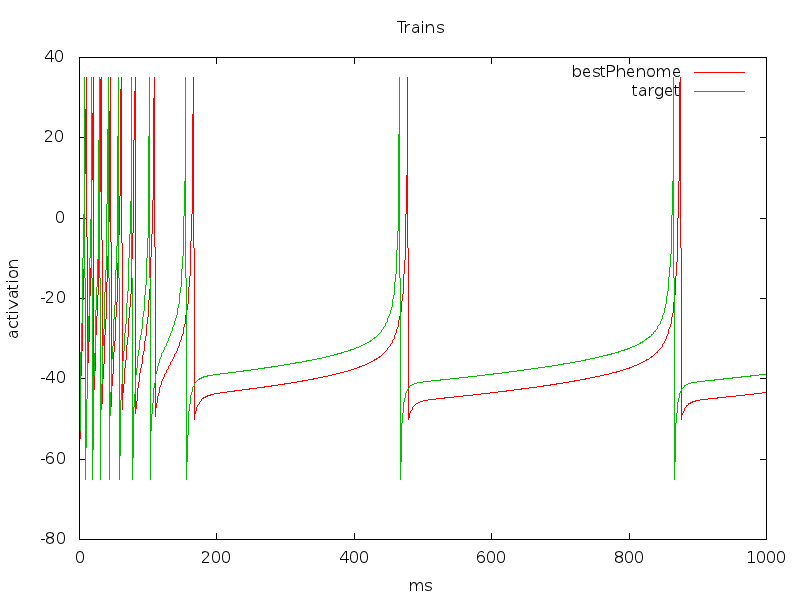
\includegraphics[width=\textwidth]{SpikeInterval-izzy4-trains-plot.png}
  \caption{Spike trains for izzy-train4 using spike interval distance measure.}
\end{figure}

\newpage

\begin{figure}[htb!]
  \centering
  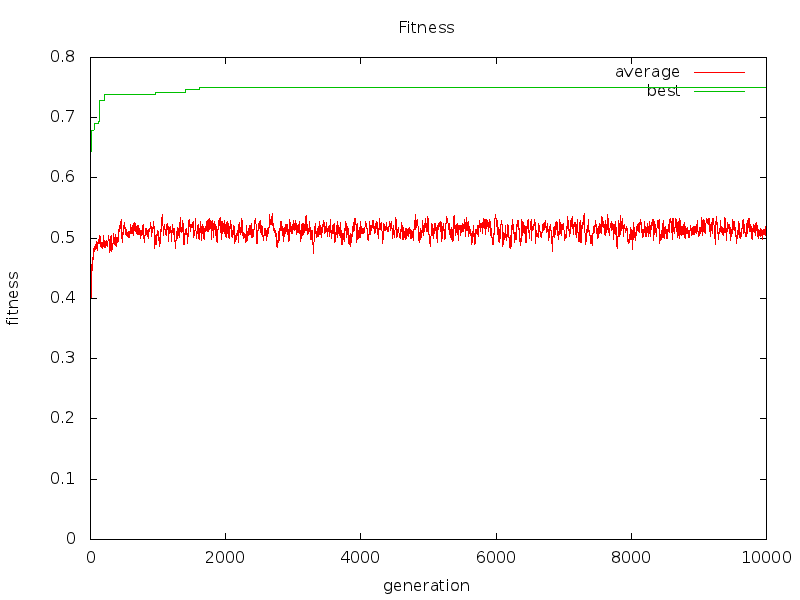
\includegraphics[width=\textwidth]{Waveform-izzy4-fitness-plot.png}
  \caption{Fitness Izzy-train4 using spike time interval distance measure.}
\end{figure}

\begin{figure}[htb!]
  \centering
  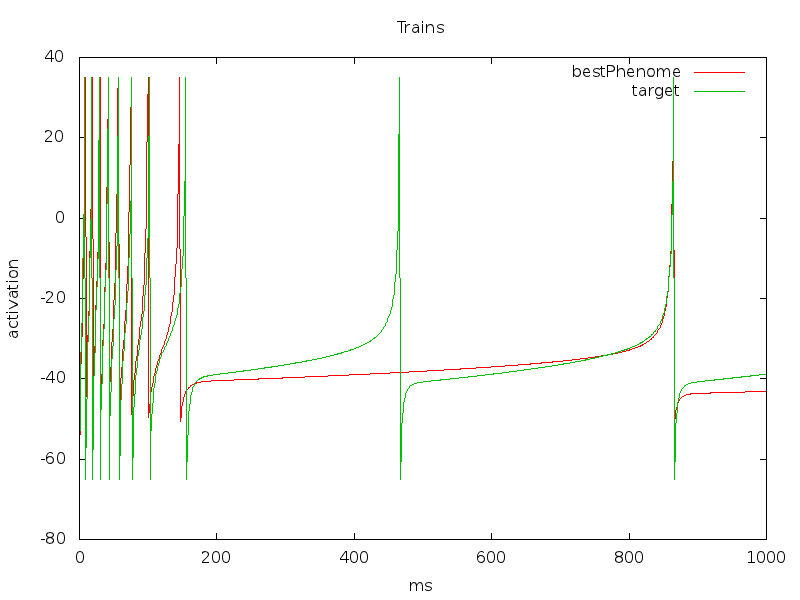
\includegraphics[width=\textwidth]{Waveform-izzy4-trains-plot.png}
  \caption{Spike trains for izzy-train4 using spike interval distance measure.}
\end{figure}

\newpage
\section{Discussion}
\label{sec:discussion}

The results we achieved are far from satisfying. The system seems to work, but our diagnosis--which we made rather early on--is that it gets stuck in local maxima in the search space. What we experienced in most of our runs was that the \textit{average} and \textit{max} fitness quickly converge and then never moved. This means a single solution dominated completely and we were unable to leave the local maxima and move on to the global maximum value.We consistently arrived at the same solutions, the parameters were nearly identical, and the plot of the spike trains looked identical.

Our solution was to add \textit{age-based filtering}. That way--we reasoned--we could kill off the stale solutions. We combined this with elitism of course, to make sure we didn't lose the progress we'd made thus far. Our hope was that we would use elitism and the creation of new children for \textit{exploitation} and use age-based filtering, and replacement with random individuals, for \textit{exploration} in order to  overcome our issues with getting stuck in local maxima.

The results were mixed, there was some improvement, but far from what we expected. It definitely looks a bit weird when we plot the average fitness and don't see much improvement, but we've experimented with a \textbf{maxAge} as low as 10. This means that each solution only survives for 10 generations, unless it gets caught by \textit{elitism}, and then replaced by another randomly generated solution.

Our next guess was that perhaps the similar solutions were dominating completely during parent selection. To remedy this we implemented a stochastic version of tournament selection where the probability that the best individual, on the tournament roster, gets picked is $p$, the second best is $p*(1-p)^2$ the third one $p*(1-p)^3$ etc. We used $p = 0.6$ for most of our runs. The effect of this change was also positive, but not monumental.

The use of \textit{age-based filtering} of course only applies when using \textit{generational mixing} as the adult selection mechanism. Even when we used \textit{age-based filtering} and turned off \textit{elitism} were we unable to escape from the local maxima; the children created from this solution were quickly able to reproduce and mutate to recreate the solution we were hoping to discard.

We've been through the entire system--some of it several times--during these last two days, but we've been unable to find any bugs or mistakes which would explain our inability to get a perfect match with the target spike trains. Nonetheless, this constant scrutiny of the systems, and of the evolutionary metaphor used, has been a great learning experience. We've probably learned quite a bit more than if the system just spat out the 12 graphs during the first 150 generations of the first 12 runs.

\subsection{Genotype to phenotype mapping}
\label{sec:genotype-phen-mapp}

The two dimensions development distance and genotype-space to phenotype-space correlation are commonly used to discuss the genotype to phenotype mapping. The correlation refers to how movements in genotype space maps to movements in phenotype space. If the correlation is great then a small change to the genotype will exhibit a small change in the expressed phenotype. If the correlations is weak, however, a small change in the genotype might result in a large change in the phenotype and thus a large change in fitness.

We most likely experienced problems relating to the phenotype-space to genotype-space correlation. What we needed was a large change in genotype in order to create a relatively small change in phenotype. This proved very difficult to achieve. For instance, we saw several times that we had matched the target spike train perfectly, except for a small offset. This small offset, in phenotype space, most likely corresponded to a huge change in genotype space, and we were unable to take the intermediary steps without being punished severely for having too low fitness.

In retrospect, perhaps we should have included a bit more redundancy in our genotype to phenotype mapping to allow for neutral mutations, that way we could develop sub-solutions without being thrown out of the population

If the development distance is short, very little effort is spent moving from genotype to phenotype. In project one there was a direct mapping from genotype to phenotype. In this project, however, the computational distance might be short, but the semantic distance is far greater. This is important because when the mapping is indirect, greater care must be taken to ensure that the mapping is complete. That a mapping is complete means that all parts of the solution space is reachable. As an aside it should be mentioned that if one has sufficient domain knowledge one might create an incomplete mapping focusing only on the areas of the solution space where the solution is known to be.

\subsection{Practical implications}
\label{sec:pract-impl}

A computational neuroscientist might have discovered a few key parameters during her research. Perhaps she has created a model to model a neuron using these key parameters. Her job now, which our tool can aid her with, is to find appropriate values for the parameters of the model.

If the computational neuroscientist has even further computational resources available she might even choose to evolve the model itself. This would amount to two levels of evolution where she one the top level has a population of models, and then on the second level uses evolution select the optimal values for the parameters of the models on level one. This would incredibly computationally intensive, but if she feels this is the only way to advance her research, she might apply for time on the university mainframe.

\section{Conclusion}
\label{sec:conclusion}

Our results were pretty good, but we weren't quite able to match the target spike trains perfectly. The learning experience induced by this failure; how we ended up questioning \emph{everything} was probably more valuable than having prettier graphs when delivery time came due.

The balance between \textit{exploitation} and \textit{exploration} can be fickle at times and we frequently questioned whether the parameters were poor or if there might be some bug in the system. We ended up focusing on \textit{exploration}, at least in the graphs shown here, as that produced somewhat better results for this assignment.

We've also been over the system with a fine-toothed comb and it should be far more robust now. Hopefully we'll have further opportunities to work with this system.
\end{document}
